\documentclass[mode=present, paper=A4paper, orien=landscape, style=default]{beamer}

\usepackage[utf8]{inputenc}
\usepackage[T1]{fontenc}
\usepackage[czech]{babel}
\usepackage{listings}
\usepackage{hyperref}
\usepackage{url}
\urlstyle{same}
\usetheme{EastLansing}
\transblindshorizontal

\title{Typografie a publikování -- Projekt č. 5\\
	\large Datové struktury}
\author{Václav Valenta}
\institute{xvalen29@stud.fit.vutbr.cz}
\date{2021}

\begin{document}
\frame{\titlepage}

%Motivace
\begin{frame}
	\frametitle{Datové struktury - motivace}
	\uv{\texttt{Bad programmers worry about the code.
	Good programmers worry about data structures and their relationships.}}\\
	\smallskip Linus Torvalds
\end{frame}
	
%Datové struktury
\begin{frame}
	\frametitle{Datové struktury}
	Programové konstrukce pro správu dat v počítačovém softwaru.\\
	Umožňují reprezentovat, ukládat a zpracovávat data\\
	Dělení datových struktur:
	\bigskip
	\begin{itemize}
		\item \textbf{Základní}\\
		proměnná, pole, struktura, objekt
		\item \textbf{Odvozené}\\
		seznam, strom, zásobník, fronta, hash tabulka, slovník, ...
	\end{itemize}
\end{frame}	

%Kritéria pro výběr vhodné datové struktury	
\begin{frame}	
	\frametitle{Kritéria pro výběr vhodné datové struktury}
	\begin{itemize}
		\item \textbf{rychlost čtení} - včetně nalezení dat
		\item \textbf{rychlost zápisu} - operace insert, delete, update
		\item \textbf{paměťová náročnost}
		\item \textbf{náročnost implementace}
	\end{itemize}
\end{frame}

%Zásobník
\begin{frame}
	\frametitle{Zásobník (Stack)}
	\begin{itemize}
		\item varianta seznamu
		\item prvky jsou uloženy lineárně za sebou
		\item každý prvek má relativní pozici (n-tý prvek seznamu)
		\item pracovat lze pouze s prvkem, který je na vrcholu zásobníku
		\item typ LIFO (Last In - First Out)
	\end{itemize}
\end{frame}

%Operace zásobníku
\begin{frame}
    \frametitle{Operace zásobníku}
    \begin{itemize}
        \item \textbf{push} - uložení prvku na vrchol zásobníku
        \item \textbf{pop} - odebrání prvku z vrcholu zásobníku
        \item \textbf{top} - vrací prvek na vrcholu zásobníku (neodebere jej)
        \item \textbf{is empty} - příznak prázdného zásobníku
        \item \textbf{size} - velikost zásobníku
    \end{itemize}
\end{frame}

%Příklad - inicializace stacku
\begin{frame}[fragile]
	\frametitle{Příklad - inicializace zásobníku}  
	\begin{verbatim}
		// Struktura 'S' reprezentující zásobník
		struct S {
		    int top;
		    unsigned size;
		    int* array;
		};
		
		// Funkce 'createStack' vytvoří zásobník velikosti 'size'
		struct S* createStack(unsigned size){
		    struct S* stack = (struct S*)malloc(sizeof(struct S));
		    stack -> size =sizep;
		    stack -> top = -1;
		    stack -> array = (int*)malloc(stack -> size*sizeof(int));
		    return stack;
		}
	\end{verbatim}
\end{frame}

%Příklad - Push/Pop
\begin{frame}[fragile]
	\frametitle{Příklad - Push/Pop}  
	\begin{verbatim}
		// Funkce 'Push' přidá prvek na konec zásobníku
		void push(struct S* stack, int item){
		    if (stack -> top == stack -> size - 1)
		        return;
		    stack -> array[++stack -> top] = item;
		}
		 
		// Funkce 'Pop' vrátí prvek z konce zásobníku
		int pop(struct S* stack){
		    if (stack -> top == -1)
		        return INT_MIN;
		    return stack -> array[stack -> top--];
		}
	\end{verbatim}
\end{frame}

%Časová složitost
%Ukázka
\begin{frame}
	\frametitle{Časová složitost}
	\begin{columns}
		\begin{column}{0.6\textwidth}
		Zásobník lze implementovat pomocí paměťového pole s vrcholem na začátku\\
		\smallskip
		V této implementaci je asymptotická složitost konstantní:
			 \begin{itemize}
			    	\item \textbf{Push}: O(1)
				\item \textbf{Pop}: O(1)	
				\item \textbf{Top}: O(1)
			\end{itemize}
		\end{column}
		\begin{column}{0.4\textwidth}		
			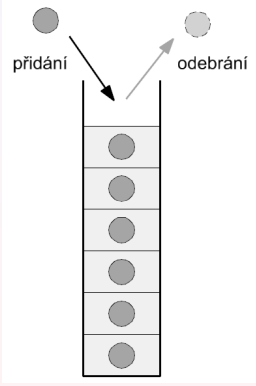
\includegraphics[scale = 0.6]{stack}
		\end{column}
	\end{columns}
\end{frame}


%Zdroje
\begin{frame}
    	\frametitle{Zdroje}
    	\texttt{\url{https://ctan.org/pkg/beamer}}\\
    	\texttt{\url{https://web.natur.cuni.cz/~bayertom/images/courses/Prog1/programovani3.pdf}}\\
	\texttt{\url{https://mirrors.nic.cz/tex-archive/macros/latex/contrib/beamer/doc/beameruserguide.pdf}}\\
	\texttt{\url{https://en.wikipedia.org/wiki/Stack_(abstract_data_type)}}\\
	\texttt{\url{https://www.geeksforgeeks.org/stack-data-structure-introduction-program}}\\
\end{frame}

\end{document}